\subsection*{Variable: CO2}
First, let us look at the product of the Haar Wavelet Transform. Figure~\ref{fig:wavelets} shows the original time series and Haar Wavelets with three different levels, 1, 2 and 10. The Weka Wavelet algorithm chooses the level from equation
\begin{align}
\mathbf{level} = \emph{ceil} \left ( \frac{\log{\emph{length}}}{\log{2}} \right ),
\end{align}
where \emph{length} is the length of the time series and \emph{ceil()} rounds the answer up to the nearest integer. When the length of the time series is about 1000 points, the equation gives 10 levels.


\begin{figure}[h!]
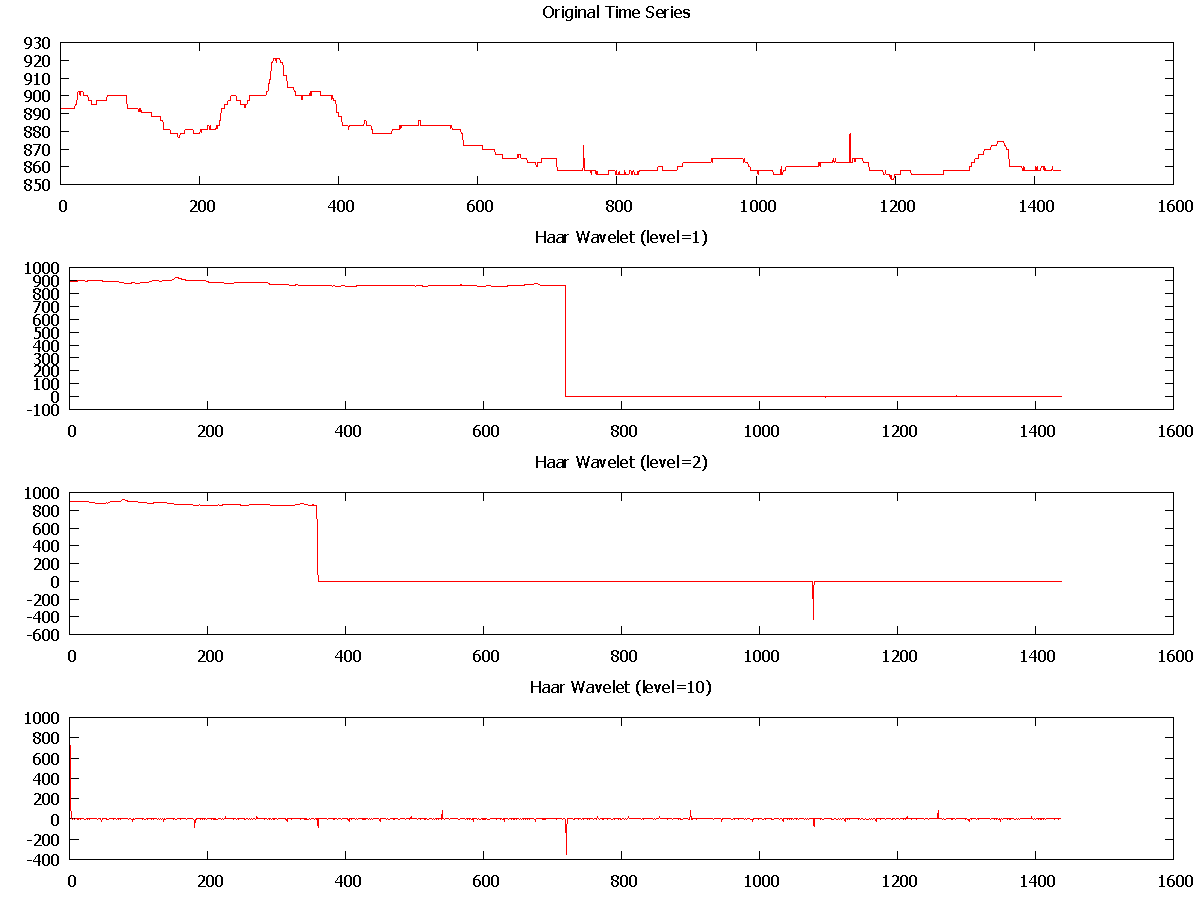
\includegraphics[scale=0.8]{images/wavelets.pdf}
\caption{Original time series and Haar Wavelets with three different levels, 1, 2 and 10.}
\label{fig:wavelets}
\end{figure}


This time the model parameters, $\gamma$ and \emph{C} should have a major impact on the classification results. Hence, we will perform an actual cross validation with 5 folds as described in Chapter 3.6.1. The data used is again from November 2012 so the resulting classifier can be compared to the one in the previous chapter.

For each parameter combination a cross validation is performed. Then, an average $AC_d$ from Equation~\ref{eq:acd} is calculated for each parameter combination. The best parameter combination is then used for training the model.

For parameter $\gamma$ the grid values are calculated using the Jaakkola Heuristics described in Equation~\ref{eq:svm_gamma} with $a_0$ set to five. This results in 11 different values for $\gamma$. For parameter \emph{C} we use a logarithmic grid $\{ 10^{i} \}$, $i = -2, ... 6$ to first find out the correct magnitude for \emph{C}.

The average accuracies and calculated $AC_d$s for \emph{C} and $\gamma$ are shown in Figures~\ref{fig:co2_svm_c} and \ref{fig:co2_svm_gamma}. Each point in the graphs is an average value of all the test runs with the given parameter value. There were a total of 55 runs for each value of \emph{C} and 45 runs for each value of $\gamma$.

\begin{center}
\begin{figure}[h!]
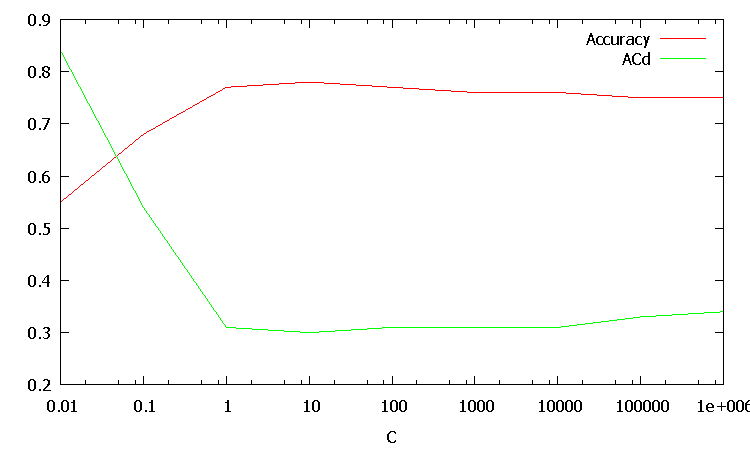
\includegraphics[scale=1.0]{images/co2_svm_c.pdf}
\caption{SVM classifier performance as a function of \emph{C}.}
\label{fig:co2_svm_c}
\end{figure}
\end{center}

\begin{center}
\begin{figure}[h!]
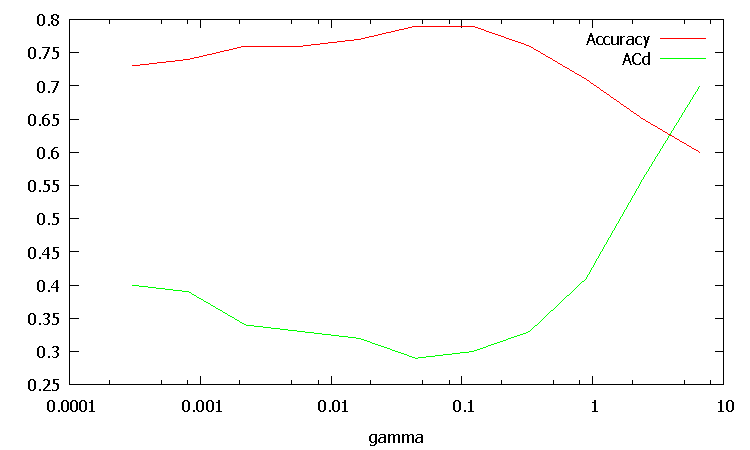
\includegraphics[scale=1.0]{images/co2_svm_gamma.pdf}
\caption{SVM classifier performance as a function of $\gamma$.}
\label{fig:co2_svm_gamma}
\end{figure}
\end{center}

The average classifier performance improves as \emph{C} increases to one. After that the accuracy decreases slowly. As the parameters might not be independent of each other, these graphs alone can not be used to select the optimal values. Figure~\ref{fig:co2_svm} shows accuracy as a function of both \emph{C} and $\gamma$. By inspecting the graphs a suitable combination for the parameters could be $C = 10$ and $\gamma = 0.05$. 

\begin{center}
\begin{figure}[h!]
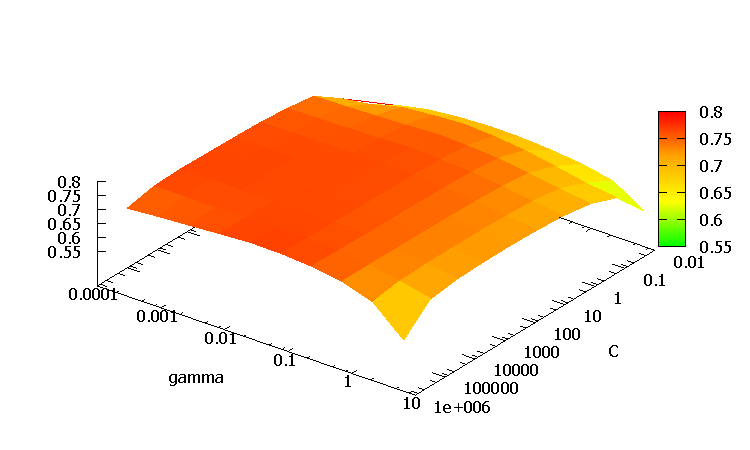
\includegraphics[scale=1.0]{images/co2_svm.pdf}
\caption{SVM classifier accuracy as a function of \emph{C} and $\gamma$.}
\label{fig:co2_svm}
\end{figure}
\end{center}

Next, the Wavelet and SVM model is trained with 14 days of data. This can not be done, however, with the same data we used for parameter selection because that approach would end up with overfitting. The values for \emph{TPR}, \emph{FPR} and Accuracy are shown in Figure~\ref{fig:co2_waveletsvm_test}.

The figure shows that the performance of this classifier varies much more than that of the DTW and kNN model.

\begin{center}
\begin{figure}[h!]
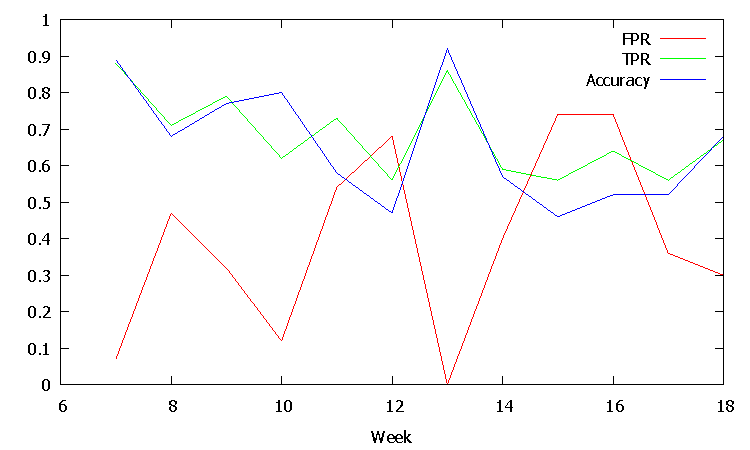
\includegraphics[scale=1.0]{images/co2_waveletsvm_test.pdf}
\caption{Wavelet and SVM based model performance with $C = 10$ and $\gamma = 0.05$.}
\label{fig:co2_waveletsvm_test}
\end{figure}
\end{center}



%\subsubsection*{Variable: VOC}
%We use the same data as for DTW and kNN based model in the %last section. Again, a grid search for optimal parameter %values is performed with data from November 2012. Since it %was shown with DTW and kNN model that the 